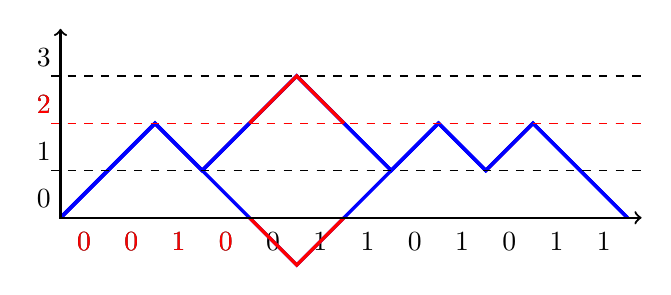
\begin{tikzpicture}[scale=.6]
    \visible<-2, 4-7>{
        \draw (.5, -.5) node {0};}
    \visible<-3, 5-7>{
        \draw (1.5, -.5) node {0};}
    \visible<-4, 6,7>{
        \draw (2.5, -.5) node {1};}
    \visible<-5,7>{
        \draw (3.5, -.5) node {0};}

    \visible<3>{
        \draw[red] (.5, -.5) node {0};}
    \visible<4>{
        \draw[red] (1.5, -.5) node {0};}
    \visible<5>{
        \draw[red] (2.5, -.5) node {1};}
    \visible<6>{
        \draw[red] (3.5, -.5) node {0};}

    \visible<-7> {
        \draw (4.5, -.5) node {0};
        \draw (5.5, -.5) node {1};
        \draw (6.5, -.5) node {1};
        \draw (7.5, -.5) node {0};
        \draw (8.5, -.5) node {1};
        \draw (9.5, -.5) node {0};
        \draw (10.5, -.5) node {1};
        \draw (11.5, -.5) node {1};}

    \visible<3>{
        \draw[red, very thick] (0, 0) -- (1, 1);
    }

    \visible<4>{
        \draw[blue, very thick] (0,0) -- (2, 2);
        \draw[red, very thick] (1, 1) -- (2, 2);
    }

    \visible<5>{
        \draw[blue, very thick] (0, 0) -- (2, 2) -- (3, 1);
        \draw[red, very thick] (2, 2) -- (3, 1);
    }

    \visible<6>{
        \draw[blue, very thick] (0, 0) -- (2, 2) -- (3, 1) -- (4, 2);
        \draw[red, very thick] (3, 1) -- (4, 2);
    }

    \visible<7>{
        \draw[blue, very thick] (0, 0) -- (2, 2) -- (3, 1) -- (5, 3) -- (7, 1) -- (8, 2) -- (9, 1) -- (10, 2) -- (12, 0);
    }

    \visible<8>{
        \draw[blue, very thick] (0, 0) -- (2, 2) -- (3, 1) -- (5, 3) -- (7, 1) -- (8, 2) -- (9, 1) -- (10, 2);
        \draw[very thick, red] (9,1) -- (10, 2);
    }
    \visible<9>{
        \draw[blue, very thick] (0, 0) -- (2, 2) -- (3, 1) -- (5, -1) -- (7, 1) -- (8, 2) -- (9, 1) -- (10, 2) -- (12, 0);
        \draw[very thick, red] (4, 0) -- (5, -1) -- (6, 0);
    }

    \visible<10>{
        \draw[blue, very thick] (0, 0) -- (2, 2) -- (3, 1) -- (5, 3) -- (7, 1) -- (8, 2) -- (9, 1) -- (10, 2) -- (12, 0);
    }


    \visible<2->{
        \draw[<->, thick] (0, 4) -- (0, 0)  -- (12.3, 0);
        \draw[dashed] (-.2, 1) -- (12.3, 1);
        \draw[dashed] (-.2, 3) -- (12.3, 3);
        \draw (0, 0) node[above left] {0};
        \draw (0, 1) node[above left] {1};
        \draw (0, 3) node[above left] {3};}
    \visible<2-9>{
        \draw (0, 2) node[above left] {2};
        \draw[dashed] (-.2, 2) -- (12.3, 2);}
    \visible<10>{
        \draw[red] (0, 2) node[above left] {2};
        \draw[red,dashed] (-.2, 2) -- (12.3, 2);
        \draw[very thick, red] (4, 2) -- (5, 3) -- (6, 2);
    }



\end{tikzpicture}